% !TeX root = writeup.tex 

\section{Results}\label{sec:results}

In order to clearly characterize the outcome of applying fairness constraints, we make the following assumption.

\begin{asm}[Institution utilities]\label{asm:institution_util}
	The institution's individual utility function is more stringent than the expected score changes, $\util(x)> 0 \implies \chg(x)>0$. (For the linear form presented in Example~\ref{ex:credit_lending},  $\frac{u_-}{u_+} < \frac{c_-}{c_+}$ is necessary and sufficient.)
\end{asm}

%This is reasonable because the institution's loss from a failure tends to be disproportionately more severe from their gains from a success, when compared to an individual's loss and gain. 
This simplifying assumption quantifies the intuitive notion that institutions take a greater risk by accepting than the individual does by applying. For example, in the credit setting, a bank loses the amount loaned in the case of a default, but makes only interest in case of a payback. Using Assumption~\ref{asm:institution_util}, we can restrict the position of $\maxprof$ on the outcome curve in the following sense.

\begin{prop}[$\maxprof$ does not cause active harm]\label{prop:mp_noharm}
	Under Assumption~\ref{asm:institution_util}, $ 0\leq \delmean^{\maxprof} \leq \delmean^*$.
\end{prop}
We direct the reader to Appendix~\ref{app:main_results_proofs} for the proof of the above proposition, and all subsequent results presented in this section. The results are corollaries to theorems presented in Section~\ref{sec:main_thm_proofs}.

%We use this assumption in our theorems, specifically to argue that $\maxprof$ does not cause active harm, which is made formal in the following proposition.Our technical results characterizing the selection rates of various fairness criteria are general and don't assume this.


%\begin{asm}[It is profitable to select $\popb$] $\accrate_\maxprof^{(\popb)} >0$
%\end{asm}
%\begin{asm}[Group $\popa$ can be harmed]
%	$\accrate_0<1$ exists for group $\popa$
%\end{asm}
%\begin{asm}[CDF domination of $\popa$ by $\popb$]\label{asm:cdf_dom}
%	%$\forall a, \sum_{x>a}\dist\supa < \sum_{x>a}\dist\supb$. Equivalently, 
%	$\forall \accrate, \RCDF\supb(\accrate)> \RCDF\supa(\accrate)$
%\end{asm}


\subsection{Prospects and Pitfalls of Fairness Criteria}
\label{sec:active_harm_fairness}
We begin by characterizing general settings under which fairness criteria act to improve outcomes over unconstrained $\maxprof$ strategies. For this result, we will assume that group $\popa$ is disadvantaged in the sense that the $\maxprof$ acceptance rate for $\popb$ is large compared to relevant acceptance rates for $\popa$.


\begin{cor}[Fairness Criteria can cause Relative Improvement]\label{cor:fairness_rel_imp}
	
	(a) Under the assumption that $\accrate\supa^{\maxprof}<\accratebar$ and $\accrate\supb^{\maxprof} > \accrate^{\maxprof}\supa$,  there exist population proportions $g_0<g_1<1$ such that, for all $\fraca \in [g_0,g_1]$, $\accrate\supa^{\maxprof}<\accrate\supa^{\dempar} < \accratebar$. That is, $\dempar$ causes relative improvement. 
	
	(b) Under the assumption that there exist $\accrate\supa^{\maxprof}<\accrate<\accrate'<\accratebar$ such that $\accrate\supb^{\maxprof} > \transfer(\accrate), \transfer(\accrate')$,
	there exist population proportions $g_2<g_3<1$ such that, for all $\fraca \in [g_2,g_3]$, $\accrate\supa^{\maxprof}<\accrate\supa^{\eqop} <\accratebar$. That is, $\eqop$ causes relative improvement.
\end{cor}


	%Assume that $\accrate\supa^{\maxprof}<\overline{\accrate}_{\maxprof}$ and $\accrate\supb^{\maxprof} > \overline{\accrate}_{\maxprof}$. Then there exist population proportion $g_0<g_1<1$ such that, for all $\fraca \in [g_0,g_1]$, $\accrate\supa^{\maxprof}<\accrate\supa^{\dempar} < \overline{\accrate}_{\maxprof}$. Instead assuming that $\accrate\supb^{\maxprof} > \transfer(\overline{\accrate}_{\maxprof})$ and further that $\accrate\supb^{\maxprof} > \transfer(\accrate)$ for some $\overline{\accrate}_{\maxprof}<\accrate<\accrate\supa^{\maxprof}$,there exist population proportion $g_2<g_3<1$ such that, for all $\fraca \in [g_2,g_3]$, $\accrate\supa^{\maxprof}<\accrate\supa^{\eqop} <\overline{\accrate}_{\maxprof}$. In these settings, fairness criteria will cause improvement for $\popa$.



%\sarah{this should go through based only on the assumption $\accrate\supb^{\maxprof} > \accrate\supa^{\maxprof}$ instead of $\accrate\supa^{\maxprof}<\bar{\accrate}_{\maxprof}$... need to adjust proof}


This result gives the conditions under which we can guarantee the existence of settings in which fairness criteria cause improvement relative to $\maxprof$. Relying on machinery proved in Section~\ref{sec:main_thm_proofs}, the result follows from comparing the position of optima on the utility curve to the outcome curve. Figure~\ref{fig:outcome_util_curves} displays a illustrative example of both the outcome curve and the institutions' utility $\Util$ as a function of the selection rates in group~$\popa$. In the utility function~\eqref{eqn:inst_util}, the contributions of each group are weighted by their population proportions $\fracj$, and thus the resulting selection rates are sensitive to these proportions.

As we see in the remainder of this section, fairness criteria can achieve nearly any position along the outcome curve under the right conditions. This fact comes from the potential mismatch between the outcomes, controlled by $\chg$, and the institution's utility $\util$.

\begin{figure}
\centering
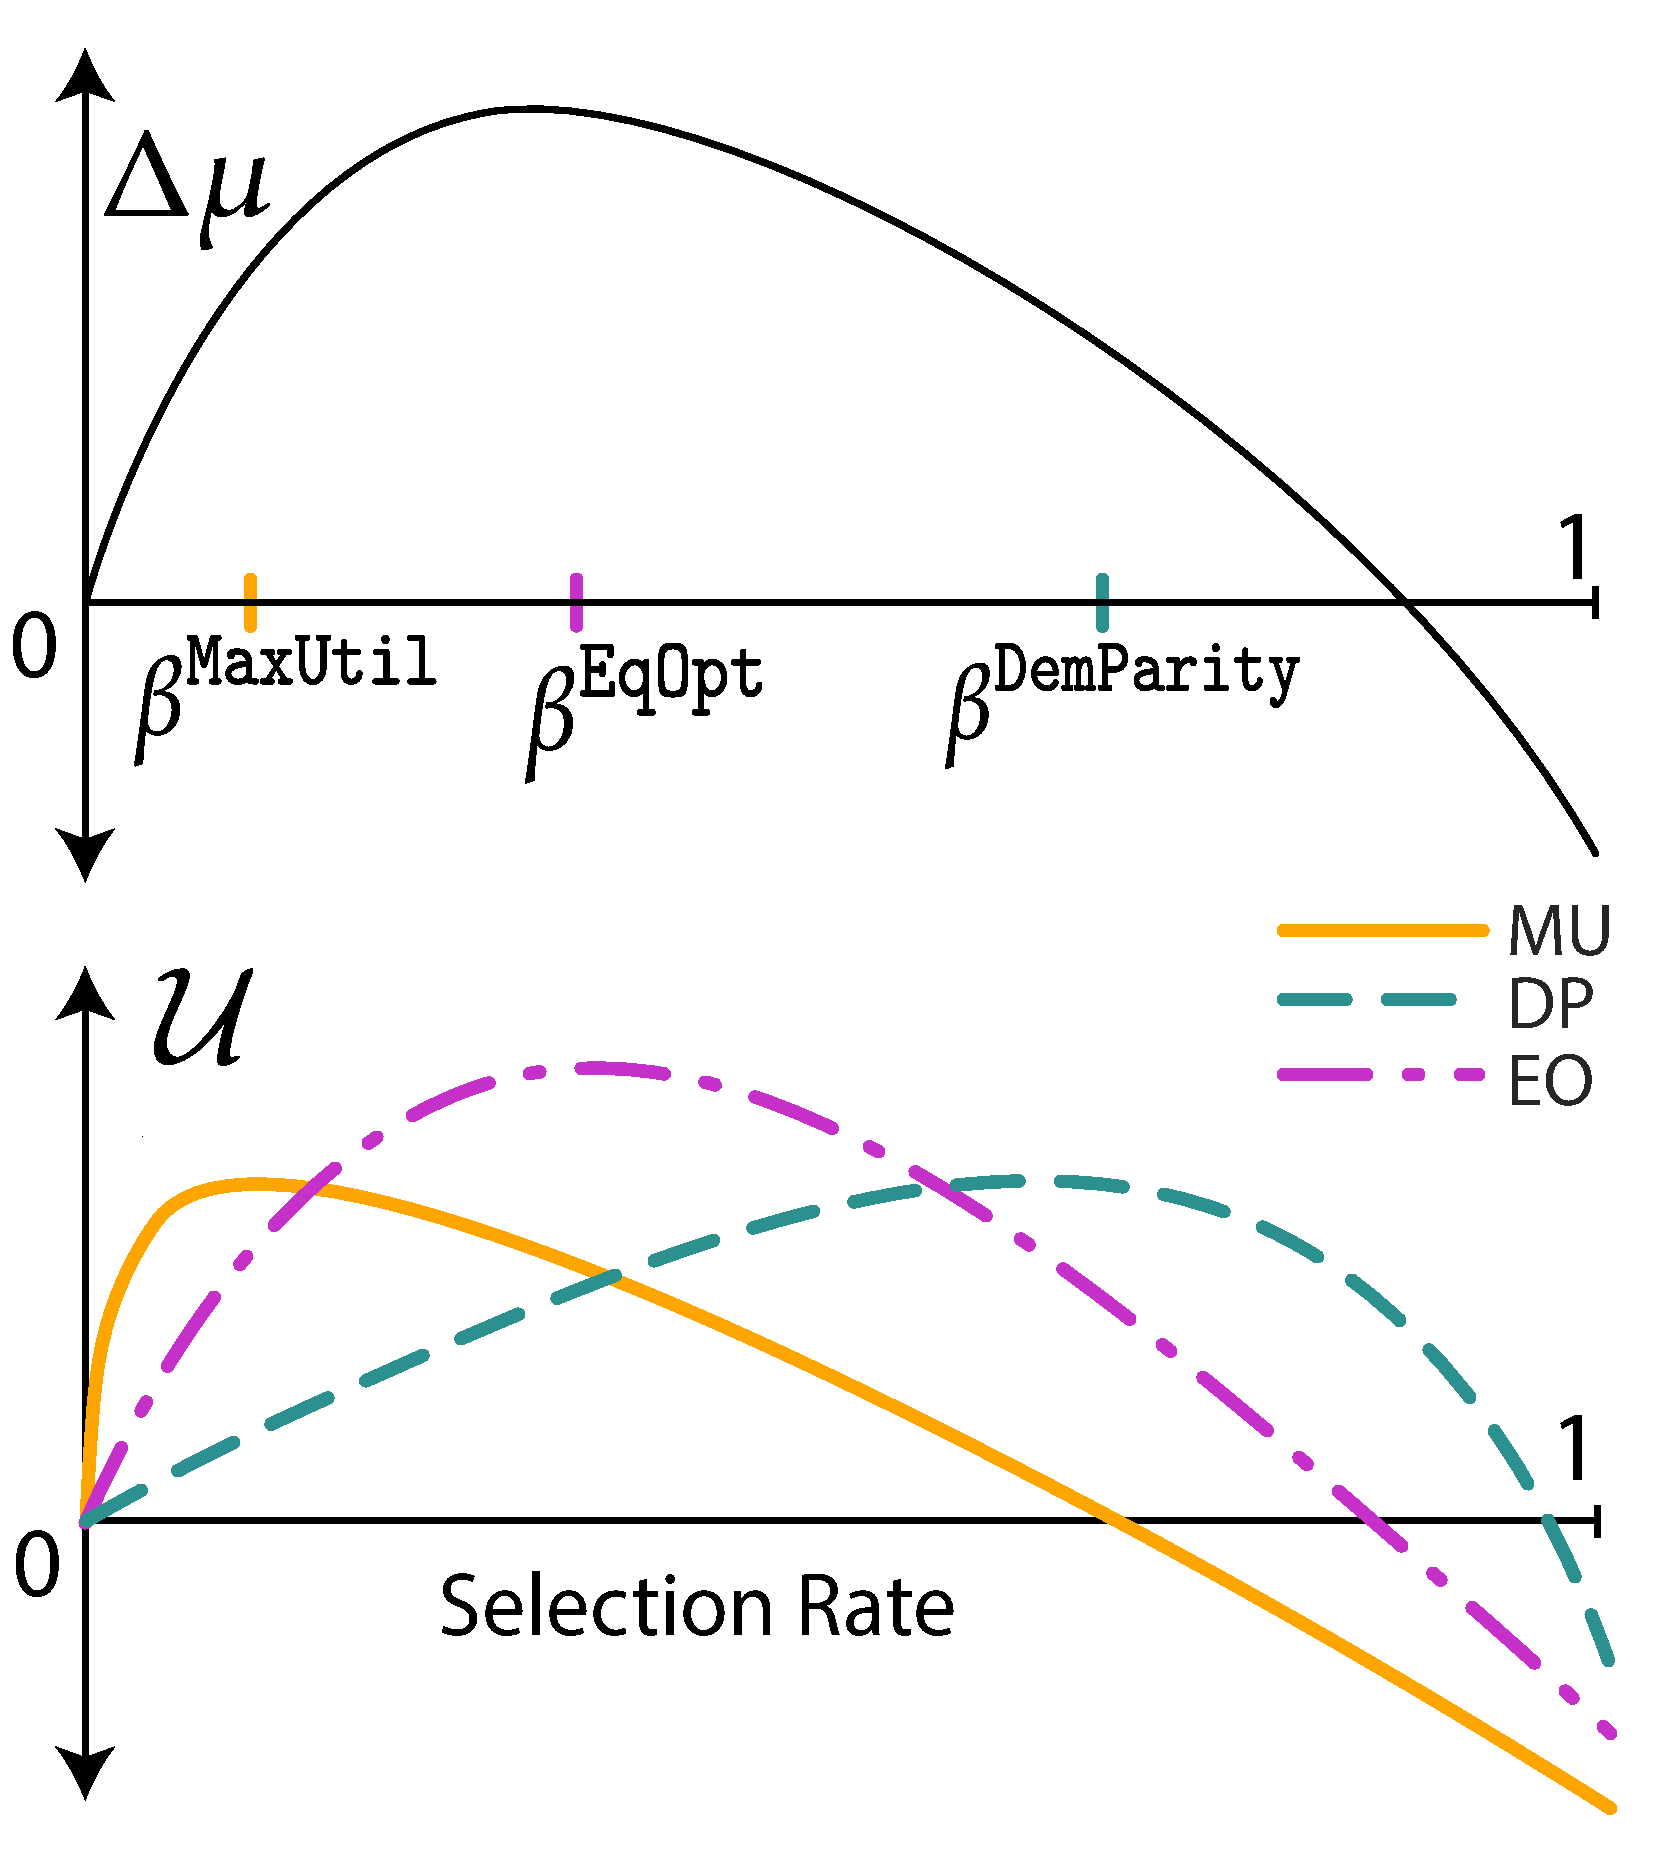
\includegraphics[width=.4\textwidth]{figures/outcome_curves/outcome_utility_curve.pdf}
\caption{Both outcomes $\delmean$ and institution utilities $\Util$ can be plotted as a function of selection rate for one group. The maxima of the utility curves determine the selection rates resulting from various decision rules.}
\label{fig:outcome_util_curves}
\end{figure}


The next theorem implies that $\dempar$ can be bad for long term well-being of the protected group by being over-generous, under the mild assumption that $\delmean\supa(\accrate\supb^{\maxprof})~<~0$:
\begin{cor}[$\dempar$ can cause harm by being over-eager] \label{cor:dp_overeager}  Fix a selection rate $\accrate$. Assume that $\accrate\supb^{\maxprof}~>~\accrate~>~\accrate\supa^{\maxprof}  $. Then, there exists a population proportion $g_0$ such that, for all $\fraca \in [0,g_0]$, $\accrate\supa^{\dempar} > \accrate$. In particular, when $\accrate=\accrate_0$, $\dempar$ causes active harm, and when $\accrate = \accratebar$, $\dempar$ causes relative harm.
\end{cor}
The assumption $\delmean\supa(\accrate\supb^{\maxprof})~<~0$ implies that a policy which selects individuals from group $\popa$ at the selection rate that $\maxprof$ would have used for group $\popb$ necessarily lowers average score in $\popa$. This is one natural notion of protected group $\popa$'s `disadvantage' relative to group $\popb$. In this case, $\dempar$ penalizes the scores of group $\popa$ even more than a naive $\maxprof$ policy, as long as group proportion $\fraca$ is small enough. Again, small $\fraca$ is another notion of group disadvantage. 

Using credit scores as an example, Corollary~\ref{cor:dp_overeager} tells us that an overly aggressive fairness criterion will give too many loans to people in a protected group who cannot pay them back, hurting the group's credit scores on average. In the following theorem, we show that an analogous result holds for $\eqop$.

\begin{cor}[$\eqop$ can cause harm by being over-eager] \label{cor:eqop_overeager} Suppose that $\accrate\supb^{\maxprof}~>~\transfer(\accrate)$ and~$\accrate~>~\accrate\supa^{\maxprof}$. Then, there exists a population proportion $g_0$ such that, for all $\fraca  \in [0,g_0]$, $\accrate^{\eqop}_{\popa}~>~\accrate$. In particular, when $\accrate~=~\accrate_0$, $\eqop$ causes active harm, and when $\accrate~=~\accratebar$, $\eqop$ causes relative harm.
\end{cor} 

We remark that in Corollary~\ref{cor:eqop_overeager}, we rely on the \emph{transfer function}, $\transfer$, which for every loan rate $\beta$ in group $\popa$ gives the loan rate in group $\popb$ that has the same true positive rate. Notice that if $\transfer$ were the identity function, Corollary~\ref{cor:dp_overeager} and Corollary~\ref{cor:eqop_overeager} would be exactly the same. Indeed, our framework (detailed in Section~\ref{sec:main_thm_proofs} and Appendix~\ref{sec:char_fairness_solns}) unifies the analyses for a large class of fairness constraints that includes $\dempar$ and $\eqop$ as specific cases, and allows us to derive results about impact on $\delmean$ using general techniques. 
In the next section, we present further results that compare the fairness criteria, demonstrating the usefulness of our technical framework.


\subsection{Comparing $\eqop$ and $\dempar$}

Our analysis of the acceptance rates of $\eqop$ and $\dempar$ in Section~\ref{sec:main_thm_proofs} suggests that it is difficult to compare $\dempar$ and $\eqop$ without knowing the full distributions $\dist\supa, \dist\supb$, which is necessary to compute the transfer function $\transfer$. In fact, we have found that settings exist both in which $\dempar$ causes harm while $\eqop$ causes improvement and in which $\dempar$ causes improvement while $\eqop$ causes harm. There cannot be one general rule as to which fairness criteria provides better outcomes in all settings. We now present simple sufficient conditions on the geometry of the distributions for which $\eqop$ is always better than $\dempar$ in terms of $\delmean\supa$.


\begin{cor}[$\eqop$ may avoid active harm where $\dempar$ fails]\label{cor:avoid_harm} Fix a selection rate $\accrate$. Suppose $\dist\supa, \dist\supb$ are identical up to a translation with $\mean\supa~<~\mean\supb$, i.e. $\dist\supa(x)~=~\dist\supb(x+(\mean\supb-\mean\supa))$. For simplicity, take $\pb(x)$ to be linear in $x$. Suppose \[ \accrate > \sum_{x > \mean \supa } \dist\supa. \] 
Then there exists an interval $[g_1, g_2]~\subseteq~[0,1]$, such that $\forall \fraca~>~g_1$, $\accrate^{\eqop}~<~\accrate$ while $\forall \fraca~<~g_2$, $\accrate^{\dempar}~>~\accrate$. In particular, when $\accrate~=~\accrate_0$, this implies $\dempar$ causes active harm but $\eqop$ causes improvement for $\fraca ~\in~[g_1, g_2]$, but for any $\fraca $ such that $\dempar$ causes improvement, $\eqop$ also causes improvement.
\end{cor} 

To interpret the conditions under which Corollary $\ref{cor:avoid_harm}$ holds, consider when we might have $\accrate_0 > \sum_{x > \mean \supa } \dist\supa$. This is precisely when $\delmean\supa( \sum_{x > \mean \supa } \dist\supa) > 0$, that is, $\delmean\supa > 0$ for a policy that selects every individual whose score is above the group $\popa$ mean, which is reasonable in reality. Indeed, the converse would imply that group $\popa$ has such low scores that even selecting all above average individuals in $\popa$ would hurt the average score. In such a case, Corollary~\ref{cor:avoid_harm} suggests that $\eqop$ is better than $\dempar$ at avoiding active harm, because it is more conservative. A natural question then is: can $\eqop$ cause relative harm by being too stingy? 

\begin{cor}[$\dempar$ never loans less than $\maxprof$, but $\eqop$ might] \label{cor:eqop_underloan} Recall the definition of the TPR functions $\tpr\supj$, and suppose that the $\maxprof$ policy $\pol^{\maxprof}$ is such that
\begin{eqnarray}
%\ratef_{\dista}(\pol^\maxprof) < \ratef_{\distb}(\pol^\maxprof) 
\accrate^\maxprof\supa < \accrate^\maxprof\supb\text{ and }
\oppa(\pol^\maxprof) > \oppb(\pol^\maxprof)
\end{eqnarray}
Then $\accrate\supa^\eqop~<~\accrate\supa^\maxprof~<~\accrate\supa^\dempar$. That is, $\eqop$ causes relative harm by selecting at a rate lower than $\maxprof$.
\end{cor}

The above theorem shows that $\dempar$ is never stingier than $\maxprof$ to the protected group $\popa$, as long as a $\popa$ is disadvantaged in the sense that $\maxprof$ selects a larger proportion of $\popb$ than $\popa$. On the other hand, $\eqop$ can select less of group $\popa$ than $\maxprof$, and by definition, cause relative harm. This is a surprising result about $\eqop$, and this phenomenon arises from high levels of in-group inequality for group $\popa$. Moreover, we show in Appendix \ref{app:main_results_proofs} that there are parameter settings where the conditions in Corollary \ref{cor:eqop_underloan} are satisfied even under a stringent notion of disadvantage we call CDF domination, described therein.



%While the last section characterized how fairness criteria compare with the unconstrained $\maxprof$ strategy, it is interesting to understand how $\eqop$ compares with $\dempar$ to contrast the different meanings of the different criteria. Theorem \ref{thm:eqopp_accrate} allows us to relate demographic parity and equal opportunity through the function $\transfer$, which we should view as a scaling function of the $\accrate$'s. \sarah{also: rescaled distributions $\dist(x)\to\frac{1}{\langle \dist,\pb\rangle}\dist(x)\pb(x)$} It also suggests that the 



\section{Relaxations of Constrained Fairness}
\subsection{Regularized fairness} 
In many cases, it may be unrealistic for an institution to ensure that fairness constraints are met exactly. However, one can consider ``soft'' formulations of fairness constraints which either penalized the differences in acceptance rate ($\dempar$) or the differences in TPR ($\eqop$). In Appendix~\ref{sec:char_fairness_solns}, we formulate these soft constraints as regularized objectives. For example, a soft-$\dempar$ can be rendered as
\begin{eqnarray}
\max_{\pol := \pola,\polb} \Util(\pol) - \lambda \Phi(\langle \dista,\pola \rangle -\langle \distb,\polb \rangle )~,
\end{eqnarray}
where $\lambda > 0$ is a regularization parameter, and $\Phi(t)$ is a convex regularization function. We show that the solutions to these objectives are threshold policies, and can be fully characterized in terms of the group-wise selection rate. We also make rigorous the notion that policies which solve the soft-constraint objective interpolate between $\maxprof$ policies at $\lambda = 0$ and hard-constrained policies ($\dempar$ or $\eqop$) as $\lambda \to \infty$. This fact is clearly demonstrated by the form of the solutions in the special case of the regularization function $\Phi(t) = |t|$, provided in the appendix.

\subsection{Fairness Under Measurement Error} 
Next, consider the implications of an institution with imperfect knowledge of scores. Under a simple model in which the estimate of an individual's score $X\sim\dst$ is prone to errors $e(X)$ such that $X~+~e(X):=\widehat X~\sim~\widehat\dst$. Constraining the error to be negative results in the setting that scores are systematically \emph{underestimated}. In this setting, it is equivalent to consider the CDF of underestimated distribution $\widehat\dist$ to be \emph{dominated} by the CDF true distribution $\dst$, that is $\sum_{x \ge c} \widehat\dist(x) \le \sum_{x \ge c} \dist(x)$ for all $c \in [\maxscore]$. Then we can compare the institution's behavior under this estimation to its behavior under the truth. 


\begin{prop}[Underestimation causes underselection]\label{prop:underestim}
Fix the distribution of $\popb$ as $\distb$ and let $\accrate$ be the acceptance rate of $\popa$ when the institution makes the decision using perfect knowledge of the distribution $\dista$. Denote $\widehat\accrate$ as the acceptance rate when the group is instead taken as $\widehat\dst\supa$. Then $\accrate\supa^\maxprof~>~\widehat\accrate\supa^\maxprof$ and $\accrate\supa^\dempar>\widehat\accrate\supa^\dempar$. If the errors are further such that the true TPR dominates the estimated TPR, it is also true that $\accrate\supa^\eqop~>~\widehat\accrate\supa^\eqop$.
\end{prop}

Because fairness criteria encourage a higher selection rate for disadvantaged groups (Corollary~\ref{cor:fairness_rel_imp}), systematic underestimation widens the regime of their applicability. Furthermore, since the estimated $\maxprof$ policy underloans, the region for relative improvement in the outcome curve (Figure~\ref{fig:outcome_curve}) is larger, corresponding to more regimes under which fairness criteria can yield favorable outcomes. Thus the potential for measurement error should be a factor when motivating these criteria.


\subsection{Outcome-based alternative} \label{sec:outcome_based}
As explained in the preceding sections, fairness criteria may actively harm disadvantaged groups. It is thus natural to consider a modified decision rule which involves the explicit maximization of $\delmean\supa$. In this case, imagine that the institution's primary goal is to aid the disadvantaged group, subject to a limited profit loss compared to the maximum possible expected profit $\Util^\maxprof$. The corresponding problem is as follows.
\begin{align}
\max_{\pola} \delmean_\popa(\pola)~~\text{s.t.}~~\Util\supa^{\maxprof} - \Util(\pol) < \delta\:.
\end{align}
Unlike the fairness constrained objective, this objective no longer depends on group $\popb$ and instead depends on our model of the mean score change in group $\popa$, $\delmean_\popa$.
\begin{prop}[Outcome-based solution]\label{prop:outcome}
In the above setting, the optimal bank policy $\pol_\popa$ is a threshold policy with selection rate $\accrate = \min\{\accrate^*, \accrate^{\max}\}$, where $\accrate^*$ is the outcome-optimal loan rate and $\accrate^{\max}$ is the maximum loan rate under the bank's ``budget''. 
\end{prop}

The above formulation's advantage over fairness constraints is that it directly optimizes the outcome of $\popa$ and can be approximately implemented given reasonable ability to predict outcomes. Importantly, this objective shifts the focus to outcome modeling, highlighting the importance of domain specific knowledge. Future work can consider strategies that are robust to outcome model errors.
